\documentclass[french,10pt,a4paper]{article}
\usepackage[T1]{fontenc}
\usepackage[left=2cm, right=2cm, top=2cm, bottom=1.5cm]{geometry}
\usepackage{graphicx}
\usepackage{mathtools}
\usepackage{amssymb}
\usepackage{amsthm}
\usepackage{thmtools}
\usepackage{xcolor}
\usepackage{nameref}
\usepackage{babel}
\usepackage{hyperref}
\title{Fiche Conversion d'énergie}
\author{Julien BLARET}
\begin{document}
	\maketitle
\section{TD1 - Alimentation d'un microprocesseur}
Ne pas confondre les sens de transistor. \newline
\begin{figure}[!h]
	\begin{minipage}{0.4\linewidth}
		\centering
		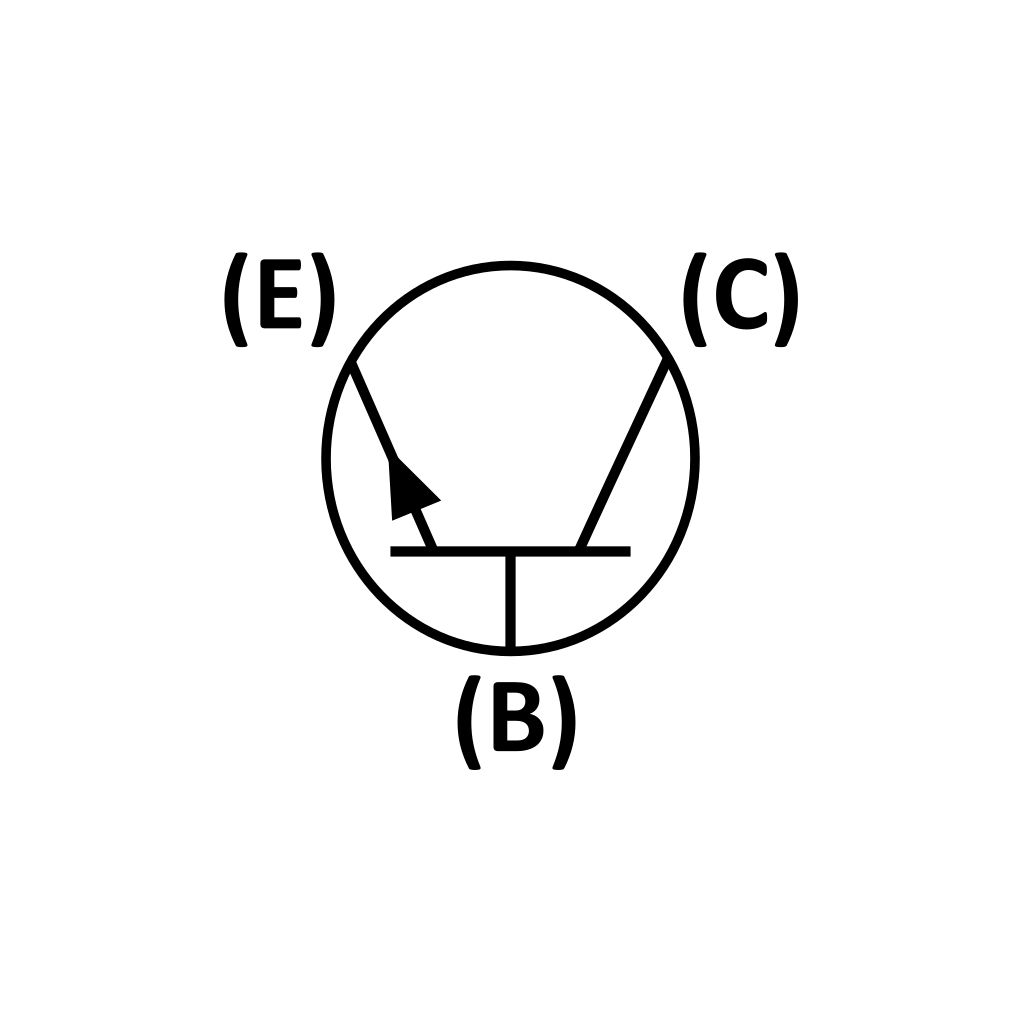
\includegraphics[width=0.7\linewidth]{NPN}
		\caption{Transistor NPN}
		\label{fig:npn}
	\end{minipage}
	\hfill
	\begin{minipage}{0.4\linewidth}
		\centering
		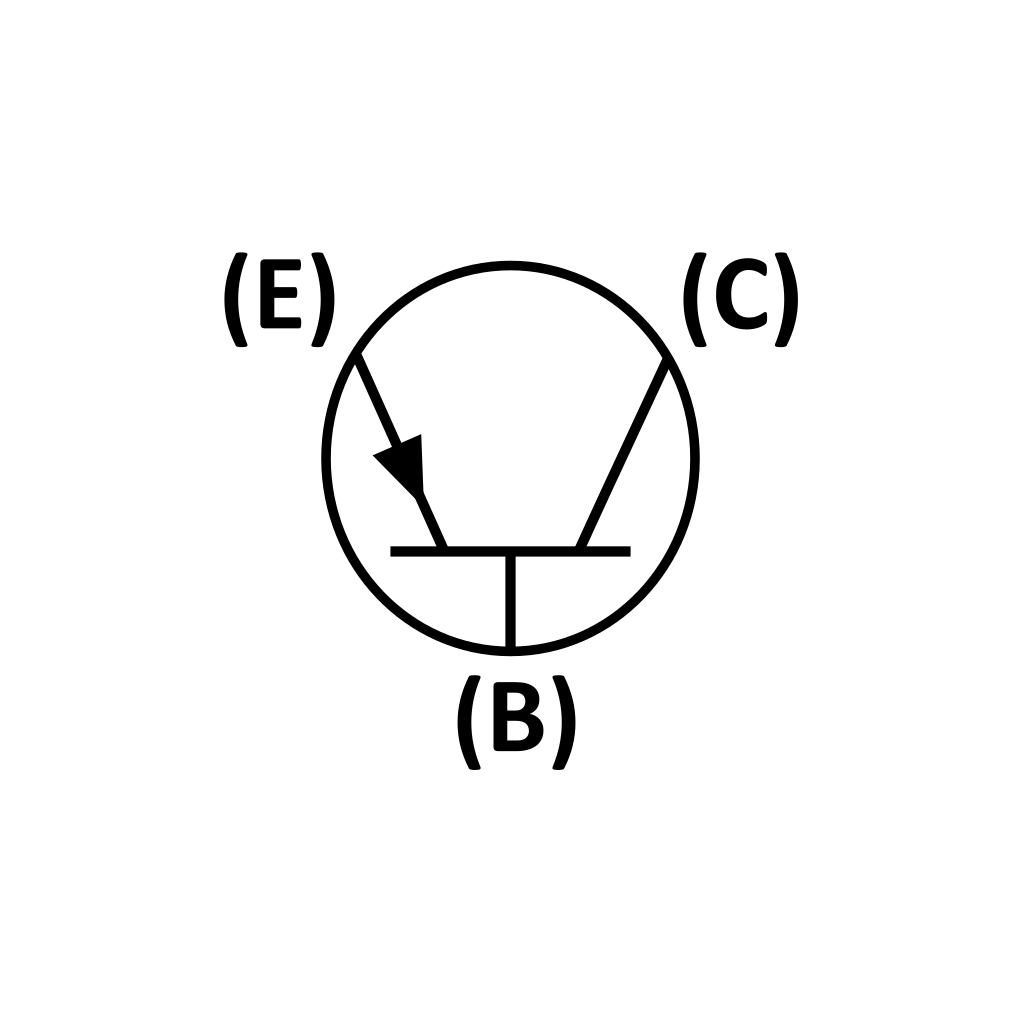
\includegraphics[width=0.7\linewidth]{PNP}
		\caption{Transistor PNP}
		\label{fig:pnp}
	\end{minipage}
\end{figure}
On n'oubliera pas non plus le schéma conventionnel du Buck:
\begin{figure}[!h]
	\centering
	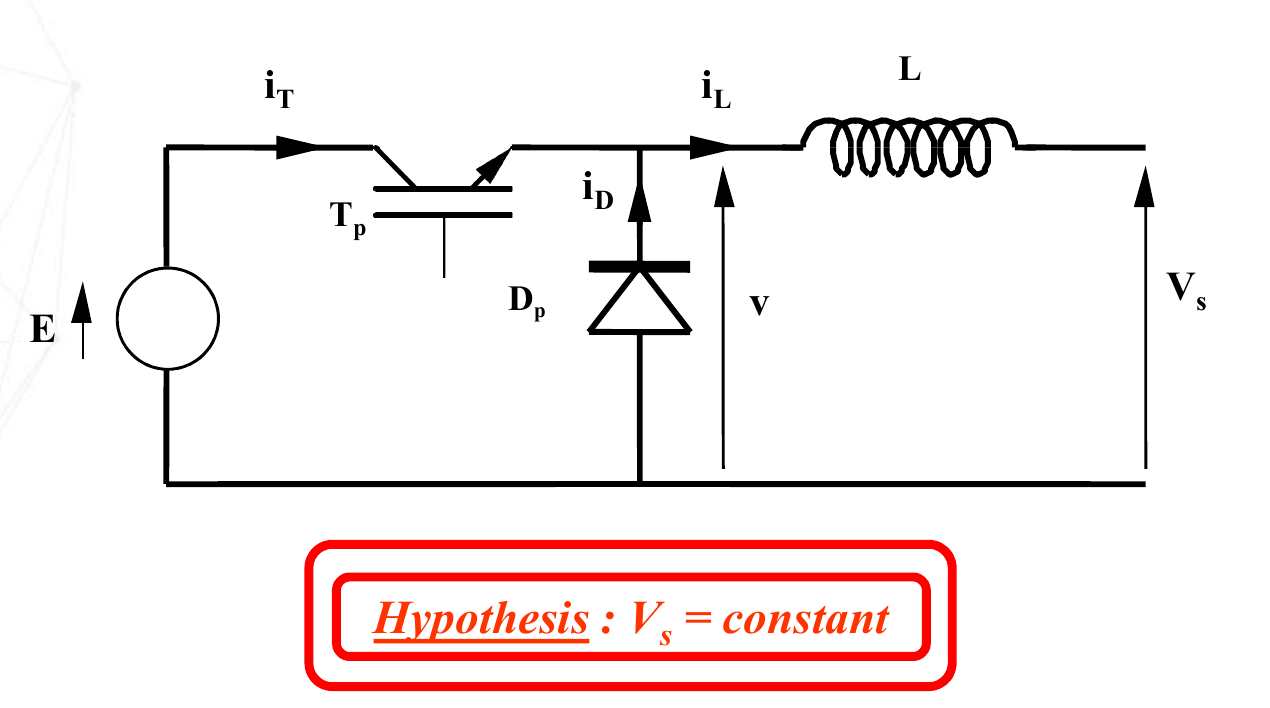
\includegraphics[width=0.7\linewidth]{Buck}
	\caption{Schéma Buck}
	\label{fig:buck}
\end{figure}
\newline Lorsque l'on demande de comparer au cahier des charges, il faut s'assurer que le composants fonctionne avec le reste du système : \textbf{\underline{relever les caractéristques éléctriques}}\newline
\begin{itemize}
	\item Faire attention à la tension de sortie minimale (valeur de FB, responsable de la commande)
	 \item Faire attention au courant de commutation max (switching limit), qui est le courant qui passe dans le transistor
\end{itemize}
Lorsque l'on calcul \textbf{l'ondulation de courant}, on se rend compte que le résultat lorsque $t\in[0,{\alpha}T]$ et $t\in[{\alpha}T, T]$ et le même au signe près. Il est donc inutile de calculer plus d'un cas.\newline\newline
Lorsque l'on calcule \textbf{l'ondulation de tension} filtrée par un condensateur, on considère uniquement \newline\underline{la partie alternative de l'intensité} : $i_C(t) = i_S(t) - I_S$. En faisant le tableau de signe de $i_S$ on a les variations de $v_S$, on peut donc trouver les extemums. La différence entre ces deux extemums est l'aire sous la courbe de $i_C(t)$, c'est à dire l'aire d'un triangle quelconque.\newline
On souvient que $g_m$ est une transconductance (en $A.V^{-1}$)
\section{TD2 }
Attention, pour trouver l'intensité passant par la charges on fait $V_{E}*I_E=I_M*U_M$\newline
Ne pas chercher compliquer pour le tram en pente et bien se concentrer sur les équations de base
\section{TD3 - BOOST}
On souvient du schéma du Boost\newline
\underline{La tension d'entrée est la moyenne de la tension de sortie}, on a donc alors $V_E = (1-\alpha)V_S$.
On peut retrouver cette équation grâce à l'ondulation de $i_L(t)$ :
\begin{itemize}
	\item Lorsque $t\in[0;{\alpha}T]$, on a $V_E = L\frac{di}{dt}$, d'où $\Delta{I} = \frac{V_E}{L}\Delta{t} = \frac{V_E}{L}{\alpha}T$
	\item Lorsque $t\in[{\alpha}T;T]$, on a $V_{S}=V_E - L\frac{di}{dt}$, d'où $\Delta{I} = \frac{V_E-V_S}{L}\Delta{t} = \frac{V_E-V_S}{L}(1-\alpha){T}$
\end{itemize}
En réunissant les deux membres on obtient l'équation aboutissant à la formule énoncée précédemment.\newline
Un tableau de contraintes est un tableau donnant  courant/tension max et moy
\section{TD4 - Half-Bridge}
Il faut faire attention aux conductions et ne pas faire le schéma à l'envers !!!! Ne pas confondre qui conduit et qui bloque en fonction des cas.\newline
Le Half-Bridge ne présenta pas de régime discontinu	
\section{TD5}
Pas besoin de faire d'intégration pour la moyenne glissante, il faut juste injecter $\alpha(t)$ dans l'équation trouvé juste avant.\newline
\end{document}